\documentclass[10pt]{memoir}
\setstocksize{220mm}{155mm} 	        
\settrimmedsize{220mm}{155mm}{*}	
\settypeblocksize{170mm}{116mm}{*}	
\setlrmargins{18mm}{*}{*}
\setulmargins{*}{*}{1.2}
%\setlength{\headheight}{5pt}%
\checkandfixthelayout[lines]
\linespread{1.16}
\flushbottom

%%% Hyphenation settings
\usepackage[htt]{hyphenat}
\hyphenation{he-lio-trope opos-sum}
\tracingparagraphs=1
%Hyphenation in Devanāgarī of the edition still missing? Probably this needs to be modified in babel-iast package? 

%%% babel
\usepackage[english]{babel}
\usepackage{babel-iast/babel-iast}

\babelfont[iast]{rm}[Renderer=Harfbuzz, Scale=1.3]{AdishilaSan}%AdishilaSan}
\babelfont[english]{rm}{Adobe Text Pro}

%%% more functionality
\PassOptionsToPackage{hyphens}{url}
\usepackage{hyperref}
\usepackage{pdflscape}
\usepackage{cleveref}
\usepackage{url}
\usepackage{cleveref}
\usepackage{microtype}
\usepackage{lineno}

%\usepackage{bigfoot}
%%% more functions
\usepackage[dvipsnames]{xcolor}
%\usepackage[para,perpage]{footmisc}

%%%für den Counter von Kapiteln und Sätzen! 
\newcommand{\uproman}[1]{\uppercase\expandafter{\romannumeral#1}}
\newcommand{\lowroman}[1]{\romannumeral#1\relax}

\makeindex
\newfontfamily\sanskritfont[Script=Devanagari,Mapping=RomDev,Scale=1.1]{Sanskrit2003}
\usepackage{pifont,fourier-orns,lettrine,psvectorian,paralist,enumitem,pdfpages,wrapfig,tabulary,lettrine,longtable}
\setlist[enumerate]{itemsep=0mm}
\usepackage[autostyle]{csquotes}
\usepackage[defaultlines=2,all]{nowidow}
\usepackage{ellipsis,adforn,booktabs,longtable,url,tikz}
\lineskiplimit=-3pt          

\makechapterstyle{IeT}{%
  \chapterstyle{default}
  \renewcommand*{\printchapternonum}{\centering}
  \renewcommand*{\clearforchapter}{\cleartorecto} 
  \aliaspagestyle{chapter}{empty}}
\chapterstyle{IeT}
\setsecnumdepth{none}  \openright  \nouppercaseheads
\settocdepth{subsubsection}

%%%% test better pagebreaks
%\def\fussy{%
%  \emergencystretch\z@
%  \tolerance 200%
%  \hfuzz .1\p@
%  \vfuzz\hfuzz}

%\interfootnotelinepenalty=10000\relax

%\usepackage[maxfloats=256]{morefloats}

%\maxdeadcycles=500

%raggedbottomsectiontrue
%%\checkandfixthelayout


%%%%%%%  biblatex
%\newcommand{\noun}[1]{\textsc{#1}}    %  philosophy-verbose
\usepackage[backend=biber, sorting=nyt, style=verbose]{biblatex} %%%%ORIGINAL TiE
\renewcommand*{\mkbibnamefamily}[1]{\textsc{#1}}


\DeclareFieldFormat{url}{%
  \mkbibacro{URL}\addcolon\space
  \href{#1}{\nolinkurl{\thefield{urlraw}}}}

\DeclareFieldFormat{citeurl}{%
  \href{#1}{\nolinkurl{\thefield{urlraw}}}} 


\DeclareFieldFormat{postnote}{#1}
\renewcommand{\postnotedelim}{, }
\addbibresource{bindu.bib}

%%% ekdosis
\usepackage[teiexport=tidy,parnotes=true]{ekdosis}% =tidy cleans up HTML and XML documents by fixing markup errors and upgrading legacy code to modern standards. parnotes=footnotes below or above critical apparatus

\SetLineation{lineation=page, modulo} %lineation=page sets thenumbering to start afresh at the top of each page. =modulo makes every fifth line numbered. {lineation=page} makes every line numbered! 

\renewcommand{\linenumberfont}{\selectlanguage{english}\footnotesize} %sets language of lines to English

\SetTEIxmlExport{autopar=false} %autopar=falseinstructs ekdosis to ignore blank lines in the.tex sourcefile as markers for paragraph boundaries. As a result, each paragraph of the edition must be found within an environment associated with the xml <p> element

\SetHooks{
  lemmastyle=\bfseries,
  %refnumstyle=\selectlanguage{english}\bfseries,
  refnumstyle=\selectlanguage{english}\color{blue}\bfseries,
  appheight=0.8\textheight,
}

\newif\ifinapparatus
\DeclareApparatus{source}[
%bhook=\inapparatustrue,
lang=english,
notelang=english,
% bhook=\selectlanguage{english},
bhook=\selectlanguage{english}\textbf{Sources:},%
%maxentries=4, 
%ehook=.]
%sep={] },
%nosep,
]

\newif\ifinapparatus
\DeclareApparatus{testium}[
%bhook=\inapparatustrue,
lang=english,
notelang=english,
% bhook=\selectlanguage{english},
bhook=\selectlanguage{english}\textbf{Testimonia:},
%maxentries=4, 
%ehook=.]
%nosep, 
]

% Declare \ifinapparatus and set \inapparatustrue at the beginning of
% the apparatus criticus block. Also set the language.  
\newif\ifinapparatus
  \DeclareApparatus{default}[
  %bhook=\inapparatustrue, 
  lang=english,
  %maxentries=33,
  %bhook=\selectlanguage{english},
  sep = {] },
  delim=\hskip 0.75em,
  rule=\rule{0.7in}{0.4pt},
]

\newif\ifinapparatus
\DeclareApparatus{philcomm}[
%bhook=\inapparatustrue,
lang=english,
notelang=english,
bhook=\selectlanguage{english}\textbf{Philological Commentary:},
%bhook=\selectlanguage{english},
sep={: },
]

\ekdsetup{
showpagebreaks,
spbmk = \textcolor{blue}{spb},
hpbmk = \textcolor{red}{hpb}
}

%\usepackage{fnpos}
%\makeFNmid
%\makeFNbottom
\usepackage[bottom]{footmisc}
%%%%%%%%%%%%%%%%%%%%%%%%%%%
\makeatletter
\def\blfootnote{\gdef\@thefnmark{}\@footnotetext}
\makeatother
%%%%%%%%%%%%%%%%%%%%%%%%%


% Macros and Definitions for the Print of Sigla
\def\acpc#1#2#3{{#1}\rlap{\textrm{\textsuperscript{#3}}}\textsubscript{\textrm{#2}}\space}
\def\sigl#1#2{{{#1}}\textsubscript{\textrm{#2}}}
\def\None{{\sigl{N}{1}}} \def\Noneac{\acpc{N}{1}{ac}\,} \def\Nonepc{\acpc{N}{1}{pc}\,}
\def\Ntwo{{\sigl{N}{2}}} \def\Noneac{\acpc{N}{2}{ac}\,} \def\Nonepc{\acpc{N}{2}{pc}\,}
\def\Done{{\sigl{D}{1}}} \def\Doneac{\acpc{D}{1}{ac}\,} \def\Donepc{\acpc{D}{1}{pc}\,}
\def\Dtwo{{\sigl{D}{2}}} \def\Dtwoac{\acpc{D}{2}{ac}\,} \def\Dtwopc{\acpc{D}{2}{pc}\,}
\def\Uone{{\sigl{U}{1}}} \def\Uoneac{\acpc{U}{1}{ac}\,} \def\Uonepc{\acpc{U}{1}{pc}\,}                 
\def\Utwo{{\sigl{U}{2}}} \def\Utwoac{\acpc{U}{2}{ac}\,} \def\Utwopc{\acpc{U}{2}{pc}\,}

%%%%%%%%%%%%%% Tattvabinduyoga - List of Witnesses   %%%%%%%%%%%%%%%%%%%
\DeclareWitness{ceteri}{\selectlanguage{english}cett.}{ceteri}[]   
\DeclareWitness{E}{\selectlanguage{english}E}{Printed Edition}[]    
\DeclareWitness{P}{\selectlanguage{english}P}{Pune BORI 664}[]  
\DeclareWitness{B}{\selectlanguage{english}B}{Bodleian 485}[]       
\DeclareWitness{N1}{\selectlanguage{english}N\textsubscript{1}}{NGMPP 38/31}[]
\DeclareWitness{N2}{\selectlanguage{english}N\textsubscript{2}}{NGMPP B 38/35}[]
\DeclareWitness{L}{\selectlanguage{english}L}{LALCHAND 5876}[]  
\DeclareWitness{D}{\selectlanguage{english}D}{IGNCA 30019}[] 
%\DeclareWitness{D2}{\selectlanguage{english}D\textsubscript{2}}{IGNCA 30020}[]  
\DeclareWitness{U1}{\selectlanguage{english}U\textsubscript{1}}{SORI 1574}[] 
\DeclareWitness{U2}{\selectlanguage{english}U\textsubscript{2}}{SORI 6082}[]
%%%%%%%%%%%%%% Tattvabinduyoga - Groups of Witnesses   %%%%%%%%%%%%%%%%%%%
\DeclareWitness{X}{\selectlanguage{english}\alpha}{Alpha Group: D,N1,N2,U1}[]
\DeclareWitness{Y}{\selectlanguage{english}\beta}{Beta Group: B,E,L,P,U2}[]
%%%%%%%%%%%%% Testimonia
\DeclareWitness{Ysv}{\selectlanguage{english}Ysv}{Yogasvarodaya}[] %%%add infos!  

%%%%%%%%%%%%%%%%%%%%%%%%%%%%%%%%%%%%%%%%%%%
% Macro for Editing Abbrevs.
\def\om{\textrm{\footnotesize \textit{om.}\ }} %prints om. for omitted in apparatus
\def\korr{\textrm{\footnotesize \textit{em.}\ }} %prints em. for emended in apparatus
\def\conj{\textrm{\footnotesize \textit{conj.}\ }} %prints conj. for conjectured in apparatus

% \supplied{text} EDITORIAL ADDITION -> Within \lem oder \rdg
% \surplus{text} EDITORIAL DELETION -> Within \lem oder \rdg
% \sic{text} CRUX
% \gap{text} LACUNAE -> [reason=??, unit=??, quantity=??, extent=??]


%%%%%%%%%%%%%%%%%%%%%%%%%%%%%%%%%%%%%%%%%%% All macros of this list can be used in 
% Macro for Editing Abbrevs.
\def\eyeskip{\textrm{{ab.\,oc. }}}
\def\aberratio{\textrm{{ab.\,oc. }}}
\def\ad{\textrm{{ad}}}
\def\add{\textrm{{add.\ }}}
\def\ann{\textrm{{ann.\ }}}
\def\ante{\textrm{{ante }}} 
\def\post{\textrm{{post }}}
%\def\ceteri{cett.\,}                   
\def\codd{\textrm{{codd.\ }}}

\def\coni{\textrm{{coni.\ }}}
\def\contin{\textrm{{contin.\ }}}
\def\corr{\textrm{{corr.\ }}}
\def\del{\textrm{{del.\ }}}
\def\dub{\textrm{{ dub.\ }}}

\def\expl{\textrm{{explic.\ }}} 
\def\explica t{\textrm{{explic.\ }}}
\def\fol{\textrm{{fol.\ }}}
\def\foll{\textrm{{foll.\ }}}
\def\gloss{\textrm{{glossa ad }}}
\def\ins{\textrm{{ins.\ }}}      
\def\inseruit{\textrm{{ins.\ }}} 
\def\im{{\kern-.7pt\lower-1ex\hbox{\textrm{\tiny{\emph{i.m.}}}\kern0pt}}} %\textrm{\scriptsize{i.m.\ }}}      
\def\inmargine{{\kern-.7pt\lower-.7ex\hbox{\textrm{\tiny{\emph{i.m.}}}\kern0pt}}}%\textrm{\scriptsize{i.m.\ }}}      
\def\intextu{{\kern-.7pt\lower-.95ex\hbox{\textrm{\tiny{\emph{i.t.}}}\kern0pt}}}%\textrm{\scriptsize{i.t.\ }}}           
\def\indist{\textrm{{indis.\ }}}  
\def\indis{\textrm{{indis.\ }}}
\def\iteravit{\textrm{{iter.\ }}} 
\def\iter{\textrm{{iter.\ }}}
\def\lectio{\textrm{{lect.\ }}}   
\def\lec{\textrm{{lect.\ }}}
\def\leginequit{\textrm{{l.n. }}} 
\def\legn{\textrm{{l.n. }}}
\def\illeg{\textrm{{l.n. }}}

\def\primman{\textrm{{pr.m.}}}
\def\prob{\textrm{{prob.}}}
\def\rep{\textrm{{repetitio }}}
\def\secundamanu{\textrm{\scriptsize{s.m.}}}            \def\secm{{\kern-.6pt\lower-.91ex\hbox{\textrm{\tiny{\emph{s.m.}}}\kern0pt}}}%   \textrm{\scriptsize{s.m.}}}
\def\sequentia{\textrm{{seq.\,inv.\ }}}  
\def\seqinv{\textrm{{seq.\,inv.\ }}}
\def\order{\textrm{{seq.\,inv.\ }}}
\def\supralineam{{\kern-.7pt\lower-.91ex\hbox{\textrm{\tiny{\emph{s.l.}}}\kern0pt}}} %\textrm{\scriptsize{s.l.}}}
\def\interlineam{{\kern-.7pt\lower-.91ex\hbox{\textrm{\tiny{\emph{s.l.}}}\kern0pt}}}   %\textrm{\scriptsize{s.l.}}}
\def\vl{\textrm{v.l.}}   \def\varlec{\textrm{v.l.}} \def\varialectio{\textrm{v.l.}}
\def\vide{\textrm{{cf.\ }}}
\def\cf{\textrm{{cf.\ }}} 
\def\videtur{\textrm{{vid.\,ut}}}
\def\crux{\textup{[\ldots]} }
\def\cruxx{\textup{[\ldots]}}
\def\unm{\textit{unm.}}
%%%%%%%%%%%%%%%%%%%%%%%%%%%%%%%%%%%%

% List of Scholars
\DeclareScholar{ego}{ego}[
forename=Nils Jacob,
surname=Liersch]

% Persons:14\DeclareScholar{ego}{ego}[15forename=Robert,16surname=Alessi]17% Useful shorthands:18\DeclareShorthand{codd}{codd.}{V,I,R,H}19\DeclareShorthand{edd}{edd.}{Lit,Erm,Sm}20\DeclareShorthand{egoscr}{\emph{scripsi}}{ego}

%Useful shorthands:
%\DeclareShorthand{codd}{codd.}{V,I,R,H}
%\DeclareShorthand{edd}{edd.}{Lit,Erm,Sm}
\DeclareShorthand{egoscr}{em.}{ego}
\DeclareShorthand{egoscrconj}{conj.}{ego}
\DeclareShorthand{egomute}{\unskip}{ego}

\usepackage{xparse}

\NewDocumentEnvironment{tlg}{O{}O{}}{\setlength{\leftskip}{0pt}\vspace{-1ex}\begin{quotation}}{\hfill #1\ \vspace{-1ex}\end{quotation}\vspace{-1ex}} %verse environment
%\NewDocumentEnvironment{tlg}{O{}O{}}{\begin{verse}}{॥#1\hskip-4pt ॥\\ \end{verse}}
\NewDocumentCommand{\tl}{m}{{\selectlanguage{iast} #1}}

\NewDocumentCommand{\extra}{m}{{\textcolor{gray}{#1}}} %command for additions to U2
\NewDocumentCommand{\crazy}{m}{{\textcolor{red}{#1}}} %totally corrupted passage
\NewDocumentCommand{\coro}{m}{{\textcolor{violet}{#1}}} %colour for sentence counter! 

\NewDocumentEnvironment{prose}{O{}}{\begin{otherlanguage}{iast}}{\end{otherlanguage}}
% \NewDocumentEnvironment{padd}{O{}}{\begin{otherlanguage}{iast}}{\end{otherlanguage}}
\NewDocumentEnvironment{tlate}{O{}}
%\NewDocumentEnvironment{tadd}{O{}}

%Define two commands: \skp ("sanskrit plus"), to be ignored by TeX in
%the edition text, but processed in the TEI output. Conversely, \skm
%("sanskrit minus") is to be processed in the edition text, but
%ignored if found in the apparatus criticus and in the TEI output:

\NewDocumentCommand{\skp}{m}{}
\TeXtoTEIPat{\skp {#1}}{#1}

%\NewDocumentCommand{\skpp}{m}{}
%\TeXtoTEIPat{\skpp {#1}}{#1}

\NewDocumentCommand{\skm}{m}{\unless\ifinapparatus#1-\fi}
\TeXtoTEIPat{\skm {#1}}{}

% \NewDocumentCommand{\dd}{}{/\hskip-4pt/}
\NewDocumentCommand{\dd}{}{\mbox{/\hskip-4pt/}}
\TeXtoTEIPat{\dd {}}{//}


%%% modify environments and commands
%%% TEI mapping
\TeXtoTEIPat{\begin {tlg}}{<lg>} %lg=(Group of verse (s)) contains one or more verses or lines of verse that together form a formal unit (e.g. stanza, chorus).
\TeXtoTEIPat{\end {tlg}}{</lg>}

\TeXtoTEIPat{\begin {prose}}{<p>}
\TeXtoTEIPat{\end {prose}}{</p>}

\TeXtoTEIPat{\begin {tlate}}{<p>}
\TeXtoTEIPat{\end {tlate}}{</p>}

\TeXtoTEIPat{\\}{}
\TeXtoTEIPat{\linebreak}{<br/>}
\TeXtoTEIPat{\noindent}{}
%\TeXtoTEI{tl}{l}
\TeXtoTEI{emph}{hi}
\TeXtoTEI{bigskip}{}
\TeXtoTEI{None}{N1}
\TeXtoTEI{Ntwo}{N2}
\TeXtoTEI{Done}{D1}
\TeXtoTEI{Dtwo}{D2}
\TeXtoTEI{Uone}{U1}
\TeXtoTEI{Utwo}{U2}
%\TeXtoTEIPat{/}{ |}
%\TeXtoTEI{//}{ ||}
\TeXtoTEIPat{\korr}{em. }
\TeXtoTEIPat{\conj}{conj.}
\TeXtoTEIPat{\om}{om.}
\TeXtoTEIPat{english}{}
\TeXtoTEIPat{\hskip}{}
\TeXtoTEIPat{\hskip-4pt}{}
\TeXtoTEIPat{\hskip-2pt}{}
\TeXtoTEIPat{-}{ }
\TeXtoTEIPat{4pt}{}
\TeXtoTEIPat{2pt}{}
\TeXtoTEIPat{\textcolor {#1}{#2}}{<hi rend="#1">#2</hi>} 

% Nullify \selectlanguage in TEI as it has been used in
% \DeclareWitness but should be ignored in TEI.
\TeXtoTEI{selectlanguage}{}



\FormatDiv{1}{\begin{center}\Large}{\end{center}}
\FormatDiv{2}{\begin{center}\small}{\end{center}}
\FormatDiv{3}{\bfseries}{.}
\title{Yogatattvabindu of Rāmacandra\\ A Critical Edition and Annotated Translation}
\date{\today}

\parindent=15pt
\begin{document}

% Zitiermöglichkeiten:
%\footcite[See][p.\,1]{goldstein01:_tibet_englis_diction_moder_tibet}
%\footnote{\cite{goldstein01:_tibet_englis_diction_moder_tibet}.}

\frontmatter
\thispagestyle{empty}
\begin{center}
  {\Large \emph{The Yogatattvabindu}}\\[3mm]
\end{center}



\newpage

\

\thispagestyle{empty}



\normalsize


\newpage


\begin{center}
\thispagestyle{empty}

\

\vskip 2mm

\begin{otherlanguage}{iast}
\LARGE \sanskritfont{Yogatattvabindu}
\end{otherlanguage}

\vskip .4cm

\Huge Yogatattvabindu \\[7mm]
\Large Critical Edition\\
with annotated Translation


\large

\vspace{3cm}

Von

Nils Jacob Liersch
\small
\vfill

\vfill

Indica et Tibetica Verlag \\ % $\cdot$ 
Marburg 2024

\vskip 6mm

\end{center}

\newpage
\newpage \ \thispagestyle{empty}
\small  \

\noindent

\
\vfill


\small
\noindent \textbf{Bibliographische Information Der Deutschen Bibliothek}

\noindent
Die Deutsche Bibliothek verzeichnet diese Publikation in der Deutschen Nationalbibliographie;
detaillierte bibliographische Informationen sind im Internet über http://dnb.ddb.de abrufbar.

\noindent
\textbf{Bibliographic information published by Die Deutschen Bibliothek}

\noindent
Die Deutsche Bibliothek lists this publication in the Deutsche Nationalbibliographie; detailed
bibliographic data is available in the Internet at http://dnb.ddb.de.  


\vskip 1cm

\noindent
\copyright\ Indica et Tibetica Verlag, Marburg 2024

\medskip

\noindent
Alle Rechte vorbehalten / All rights reserved

\medskip

\noindent
Ohne ausdrückliche Genehmigung des Verlages ist es nicht gestattet, das Werk oder einzelne Teile
daraus nachzudrucken, zu vervielfältigen oder auf Datenträger zu speichern.

\smallskip

\noindent
Apart from any fair dealing for the purpose of private study, research, criticism or review, no
part of this book may be reproduced or translated in any form, by print, photo form, microfilm, or
any other means without written permission. Enquiries should be made to the publishers.

\bigskip

\noindent
Satz: \ \ Nils Jacob Liersch \\
Herstellung: \ \ BoD – Books on Demand GmbH, Norderstedt  \\

\bigskip

\noindent
%\ISBN     

\normalsize

\newpage

%\maketitle
\clearpage
\tableofcontents
\addtocounter{page}{-1}
\thispagestyle{empty}
\clearpage


\mainmatter

\chapter{Conventions in the Critical Apparatus}
\section{Sigla in the Critical Apparatus}

\begin{itemize}
\item E : Printed Edition
\item P : Pune BORI 664
\item L : Lalchand Research Library LRL5876
\item B : Bodleian Oxford D 4587
\item \None : NGMPP B 38-31
\item \Ntwo : NGMPP B 38-35 / A 1327-14
\item \Done : IGNCA 30019
\item \Uone : SORI 1574
\item \Utwo: SORI 6082
\end{itemize}

\chapter{Critical Edition \& Annotated Translation}
\cleardoublepage
\begin{alignment}[
  texts=edition[class="edition"];
  translation[class="translation"],
  ]
  \begin{edition}
    \ekddiv{type=ed}
    \ekddiv{
      head={[\uproman{39}. \textbf{piṇḍamadhye 'ṣṭakulaparvatāḥ}]},
      type=section,
      depth=2, 
      n=XXXIX
    }
    \begin{prose}
      \noindent
%----------------------------
%idānīm             aṣṭamakulaparvatāḥ kathyante/  \E
%idānīm             aṣṭakulaparvatāḥ   kathyaṃte   \P
%idānīm             aṣṭamakulaparvatāḥ kathyaṃte// \B
%idānīm             aṣṭamakulaparvatāḥ kathyaṃte// \L
%\om                                               \N1
%idānīṃ piṃḍamadhye aṣṭakulaparvatāḥ   kathyaṃte// \D
%\om                                               \N2
%idānīṃ piṃḍamadhye aṣṭakulaparvatāḥ   kathyaṃte   \U1
%idānīm             aṣṭakulaparvatā    kathyaṃte// \U2
%-----------------------------
%Now, the eight mountains within the body are taught. 
%----------------------------
\note[type=source, labelb=281, labele=_281e, nosep]{cf. YSv (PT p. 843): idānīṃ parvatāś cāṣṭau kathyante śṛṇu yatnataḥ | merudaṇḍe sumerus tu pīṭhamadhye himālayaḥ | vāmaskandhe tathā dakṣe malayo mandarācalaḥ | vindhyas tu dakṣiṇe karṇe vāme maināka īśvari | lalāṭe madhyadeśe tu śrīśailaḥ parameśvari | tathā brahmakapāṭasthaḥ kailāsaḥ parvato mahān | sumerur himavān vindhyo malayo mandaras tathā | śrīśailo mainākaś ceti kailāso 'ṣṭau ca parvatāḥ | apare parvatāḥ sarveaṅgulīmadhyavāsinaḥ |}
\note[type=source, labelb=282, labele=_281e, nosep]{cf. SSP 3.10 (Ed. p. 56): meruparvato merudaṇḍe vasati | kailāso brahmakapāṭe vasati | himālayaḥ pṛṣṭhe | malayo vāmakandhare | mandaro dakṣiṇakandhare | vindhyo dakṣiṇakarṇe | maināko vāmakarṇe | śrīparvato lalāṭe | evam aṣṭa kulaparvatāḥ | anye upaparvatāḥ sarvāṅguliṣu vasanti |}
  \app{\lem[wit={D,U1}]{idānīṃ}
  \rdg[wit={ceteri}]{idānīm}}
\app{\lem[wit={D,U1}]{piṇḍamadhye}
  \rdg[wit={ceteri}]{\om}}
\app{\lem[type=emendation, resp=egoscr]{'ṣṭakulaparvatāḥ}
  \rdg[wit={P,D,U1}]{aṣṭakulaparvatāḥ}
  \rdg[wit={U2}]{aṣṭakulaparvatā}
  \rdg[wit={B,E,L}]{aṣṭamakulaparvatāḥ}}
kathyante/
%----------------------------  
%merudaṇḍamadhye merumaṃdaraḥ/   brahmakapāṭamadhye  kailāsaḥ/ \E
%merudaṇḍamadhye merumaṃdaraḥ    brahmakapāṭamadhye  kailāsaḥ  \P
%merudaṇḍamadhye merumaṃdaraḥ/   brahmakapāṭamadhye  kailāsaḥ/ \B
%merudaṇḍamadhye merumaṃdaraḥ/   brahmakapāṭamadhye  kailāsaḥ/ \L
%\om                                                                  \N1
%merudaṃḍamadhye merumparvataḥ// brahmakapāṭamadhye  kailāsaparvataḥ \D
%\om                                                                 \N2
%merudaṇḍamadhye merumparvattaḥ  brahmakapāṭamadhye  kailāsaparvataḥ \U1
%merudaṇḍamadhye merumaṃdaraḥ//  brahmakapāṭamadhye  kailāsaḥ// \U2 %%%419.jpg 
%-----------------------------
%(1) Within the spine is mount Meru. (2) Within the door of Bahman is mount Kailasa. 
%----------------------------
merudaṃḍamadhye
\app{\lem[type=emendation, resp=egoscr]{meruparvataḥ}
  \rdg[wit={D,U1}]{merumparvataḥ}
  \rdg[wit={ceteri}]{merumaṃdaraḥ}}\dd{}
brahmakapāṭamadhye
\app{\lem[wit={D,U1}]{kailāsaparvataḥ}
  \rdg[wit={ceteri}]{kailāsaḥ}}\dd{}
%----------------------------
%pṛṣṭhamadhye   himācalaḥ/           vāmaskandhe malayācalaḥ/  dakṣiṇaskandhe mandarācalaḥ/  dakṣiṇakarṇe vindhyācalaḥ/  \E
%pṛṣṭhaṃ madhye himācalaḥ            vāmaskaṃdhe malayācalaḥ   dakṣiṇaskaṃdhe maṃdarācalaḥ   dakṣiṇakarṇe vindhyācalaḥ    \P
%pṛthvīmadhye  himācalaḥ/            vāmaskaṃdhe malayācalaḥ/  dakṣiṇaskaṃdhe maṃdarācalaḥ/  dakṣiṇakarṇe vindhyācalaḥ/ \B
%pṛthvīmadhye   himācalaḥ/           vāmaskaṃdhe malayācalaḥ/  dakṣiṇaskaṃdhe maṃdarācalaḥ/  dakṣiṇakarṇe viṃdhyācalaḥ/  \L
%\om                                                                 \N1
%paiṭimadhye    himācalaḥ// parvataḥ vāmaskaṃdhe malayācalaḥ   dakṣaṇaskaṃdhe maṃdarācalaḥ   dakṣaṇakarṇe viṃdhyācalaḥ  \D
%\om                                                                 \N2
%paiṭhamadhye   himācala----parvataḥ vāmaskaṃdhe malayācalaḥ   dakṣaṇaskaṃdhe maṃdarācalaḥ   dakṣaṇakarṇe viṃdhyācalaḥ  \U1
%pṛṣṭhamadhye   himācalaḥ//          vāmaskandhe malayācalaḥ// dakṣiṇaskandhe mandarācalaḥ// dakṣiṇakarṇe vindhyācalaḥ//  \U2
%-----------------------------
% (3) Within the back is the Himālaya. (4) Within the left shoulder mount Malabar. (5) Within the right shoulder the mountain of Mandara. (6) In the right ear the Vindhya mountain. 
%----------------------------
\app{\lem[wit={E,U2}, alt={pṛṣṭhamadhye}]{pṛṣṭha:\\madhye}
  \rdg[wit={P}]{pṛṣṭhaṃ madhye}
  \rdg[wit={B,L}]{pṛthvīamadhye}
  \rdg[wit={D}]{paiṭimadhye}
  \rdg[wit={U1}]{paiṭhamadhye}}
\app{\lem[wit={ceteri}]{himācalaḥ}
  \rdg[wit={D}]{himācalaḥ || parvataḥ}
  \rdg[wit={U1}]{himācalaparvataḥ}}\dd{}
vāmaskaṃdhe malayācalaḥ\dd{}
dakṣiṇaskaṃdhe maṃdarācalaḥ\dd{}
dakṣaṇakarṇe viṃdhyācalaḥ\dd{}
%----------------------------
%vāmakarṇe mainākaḥ/  lalāṭamadhye śrīśailaḥ/   apare śailāḥ   hastayoḥ  pādayor aṃgulīnāṃ   mūleṣu varttaṃte// \E
%vāmakarṇe mainākaḥ   lalāṭamadhye śrīśailaḥ    apare śailā    hastayoḥ  pādayor aṃgulīnāṃ   mūleṣu varttaṃte   \P
%vāmakarṇe mainākaḥ/  lalāṭamadhye śrīśailāsaḥ/ apare śailā    hastayoḥ/ pādayor aṃguli------mūleṣu vartate//   \B
%vāmakarṇe mainākaḥ/  lalāṭamadhye śrīśailaḥ/   apare śailā    hastayoḥ/ pādayor aṃgulī------mūleṣu vartate/    \L
%\om                                                                 \N1
%vāmakarṇe mainākaḥ// lalāṭamadhye śrīśailaḥ//  apare parvatāḥ hastayoḥ  pādayor aṃgulīnāṃ   madhye vartatte//  \D
%\om                                                                 \N2 
%vāmakarṇe mainākaḥ   lalāṭamadhye śrīśailaḥ    apare parvatāḥ hastayoḥ  pādayor aṃgulībhyāṃ madhye parvate     \U1
%vāmakarṇe mainākaḥ   lalāṭamadhye śrīśailaḥ//  apare śailāḥ// hastayoḥ  pādayor aṃgulīnāṃ   mūleṣu vartaṃte//  \U2
%-----------------------------
% (7) In the left ear the Maināka[-mountain]. (8) Within the forehead Śrīśaila. Other mountains exist in the hands, feet, and toes. 
%----------------------------
vāmakarṇe mainākaḥ\dd{}
lalāṭamadhye
\app{\lem[wit={ceteri}]{śrīśailaḥ}
  \rdg[wit={B}]{śrīśailāsaḥ}}/ 
apare \app{\lem[wit={D,U1}]{parvatāḥ}
  \rdg[wit={E,U2}]{śailāḥ}
  \rdg[wit={B,P,L}]{śailā}}
pādayo\skp{r-aṃ}\app{\lem[wit={E,P,D},alt={aṃgulīnāṃ}]{\skp{r-aṃ}gulīnāṃ}
  \rdg[wit={U1}]{aṃgulībhyāṃ}
  \rdg[wit={B,L}]{aṃguli°}}
\app{\lem[wit={ceteri}]{mūleṣu}
  \rdg[wit={D,U1}]{madhye}}
\app{\lem[wit={ceteri}]{vartante}
  \rdg[wit={B,L}]{vartate}
  \rdg[wit={U1}]{parvate}}/\linelabel{_281e}
\end{prose}
\ekddiv{
  head={[\uproman{40}. \textbf{śarīre navanāḍyaḥ}]},
  type=section,
  depth=2, 
  n=XL
}
\label{ninerivers}
    \begin{prose}
      \noindent
%----------------------------
%idānīṃ śarīramadhye navanāḍyas tiṣṭhanti   tanmadhye navanadīnāṃ     sthānāni   varttante/   \E
%idānīṃ śarīre       navanaḍyas tiṣṭhaṃti   tanmadhye navāṃnā nadīnāṃ sthānāni   vartaṃte     \P
%idānīṃ śarīre       navanaḍyas tiṣṭhanti// tanmadhye navānāṃ nadīnāṃ sthānāni   vartate/     \B
%idānīṃ śarīre       navanaḍyaḥ tiṣṭhaṃti/  tanmadhye navānāṃ nadīnāṃ sthānāni   vartaṃte/    \L
%\om                                                                 \N1
%idānīṃ śarīre       ṇavānāḍyas tiṣṭhati//  tanmadhye navānāṃ nadīnāṃ sthānāni   vartraṃte//  \D
%\om                                                                 \N2
%idānīṃ śarīre       ṇavānaḍyaḥ stiṣṭhaṃti  tanmadhye navānāṃ nadīnāṃ sthānāni   vartaṃte    \U1
%idānīṃ śarīramadhye navanāḍyas tiṣṭhati//  tanmadhye navānāṃ nadīnāṃ          nivarttaṃte// \U2
%-----------------------------
%Now, within the body there are nine rivers. Within it the courses of the nine rivers exist. 
%----------------------------
      \note[type=source, labelb=284, labele=_284e, nosep]{cf. YSv (PT p. 843): śarīre navanāḍīsthā narmadā ca maheśvari | iḍāyāṃ yamunā devi piṅgalāyāṃ sarasvatī | suṣumnāyāṃ vahed gaṅgā cānyonyāsu ca nāḍiṣu | gaṅgā sarasvatī godā narmadā yamunā tathā | kāverī candrabhāgā ca vitastā ca iḍāvatī | dvisaptatisahasreṣu nadīnadaparisravaḥ |}
      \note[type=source, labelb=283, labele=_284e, nosep]{cf. SSP 3.11-12 (Ed. p. 57): pīnasā yamunā gaṅgā candrabhāgā sarasvatī | vipāsā śatarudrā ca śrīrātriś caiva narmadā | evaṃ navanadyo navanāḍīṣu vasanti | anyā upanadyaḥ kulyopakulyā dvisaptatisahasranāḍīsu vasanti |}
idānīṃ
\app{\lem[wit={ceteri}]{śarīre}
  \rdg[wit={E,U2}]{śarīramadhye}}
\app{\lem[wit={E,U2},alt={navanāḍyas}]{navanāḍya\skp{s-ti}}
  \rdg[wit={B,L,P}]{navanaḍyas}
  \rdg[wit={D}]{ṇavānāḍyas}
  \rdg[wit={U1}]{ṇavānaḍyaḥs}}
\app{\lem[wit={ceteri}]{tiṣṭhanti}
  \rdg[wit={D,U2}]{tiṣṭhati}}/
tanmadhye
\app{\lem[wit={ceteri}]{navānāṃ nadīnāṃ}
  \rdg[wit={E}]{navanadīnāṃ}}
sthānāni
\app{\lem[wit={ceteri}]{vartante}
  \rdg[wit={U2}]{nivartaṃte}
  \rdg[wit={B}]{vartate}}/
%----------------------------     
%gaṃgāyamune vitastā candrabhāgā sarasvatī vipāśā   śatahradā   irāvatī narmadā/   \E [p.52]
%gaṃgāyamunā vitastā caṃdrabhāgā sarasvatī vipāśā   śātahṛdā    irāvati narmmadā    \P
%gaṃgāyamunā vitastā caṃdrabhāgā sarasvatī vipāśā   śāśatahṛdā  irāvati narmadā/  \B
%gaṃgāyamunā vitastā caṃdrabhāgā sarasvati vipāśā   śatat hṛda  irāvati narmadā// \L
%\om                                                                 \N1
%gaṃgāyamunā vitastā caṃdrabhāgā sarasvatī/ vaipaśā śata hṛdā// irāvatī/ narmadā/ \D
%\om                                                                 \N2
%gaṃgāyamunā vitastā caṃdrabhāgā sarasvatī vaipaśā  śata hṛdā   airāvati narmadā \U1
%gaṃgāyamunā vitastā candrabhāgā sarasvatī vipāśā   śātadrumā//          narmadā   \U2
%-----------------------------
%Gaṅga, Yamuna, Vitastā, Candrabhāga, Sarasvatī, Vipāśā, Śatarudrā, Irāvati und Narmadā.  
%-----------------------------
gaṃgāyamunā vitastā caṃdrabhāgā
\app{\lem[wit={ceteri}]{sarasvatī}
  \rdg[wit={L}]{sarasvati}}
\app{\lem[wit={ceteri}]{vipāśā}
  \rdg[wit={D,U1}]{vaipaśā}}
\app{\lem[type=emendation, resp=egoscr]{śatarudrā}
  \rdg[wit={D,P,U1}]{śātahṛdā}
  \rdg[wit={E}]{śatahradā}
  \rdg[wit={B}]{śāśatahṛdā}
  \rdg[wit={U2}]{śātadrumā}}
\note[type=philcomm, labelb=285, lem={śatarudrā}]{I emended according to YSv (PT).}
\app{\lem[wit={D,E}]{irāvatī}
  \rdg[wit={B,L,P,U1}]{irāvati}
  \rdg[wit={U2}]{\om}}
narmadā/ 
%-----------------------------
%aparā    nadyo    nadāni       srotāṃsi   taṭākāni  vāpīkūpā---disaptati----sahasranāḍī----madhye tiṣṭhanti/  \E
%aparā    nadyo    nadānir jārā srotāṃsī   taṭānī    vāpīkūpā---dvisaptatī---sahasranāḍīnāṃ madhye tiṣṭaṃti    \P %7660.jpg
%aparā    nadyo    nadānir jñārāsty etāṃsī taṭānī    vāpīkūpā---dvisaptatī---sahasranāḍīnā--madhye tiṣṭaṃti/   \B
%aparā    nadyo    nadānir jñārāsty etāṃsi taṭāni    vāpīkūpā---dvisaptati---sahasranāḍīnāṃ madhye tiṣṭaṃti/   \L
%\om                                                                                                   \N1
%aparā    nadyopanadīnair   bhurasrota-----taṭāka----vāpikupāḥ  dvisaptati---sahasranāḍīnāṃ madhye tiṣṭaṃti/  \D
%\om                                                                                                   \N2
%gaṃḍakī  nadyūpanadīnair  bhurasrota------taḍaga    vāpīkūpa---dvisaptati---sahastranāḍī   madhye  tiṣṭhaṃṭī  \U1  %em zu upanadinirjhara!!! Wasserfälle! 
%aparā    nadyo   nadānir  jñārāsrotāsī    taṭhānī   vāpīkūpā---dvisaptati---sahasranāḍīnāṃ madhye tiṣṭaṃti//  \U2
%-----------------------------
%Other rivers, and waterfalls near the rivers, currents, lakes, ponds and wells are situated within the 72000 channels.
%-----------------------------
\app{\lem[wit={ceteri}]{aparā}
  \rdg[wit={U1}]{gaṃḍakī}}
\app{\lem[type=emendation, resp=egoscr]{nadyopanadinirjharāḥ srotāṃsi}
    \rdg[wit={D}]{nadyopanadīnairbhurasrota°}
    \rdg[wit={U1}]{nadyūpanadīnairbhurasrota°}
    \rdg[wit={P}]{nadyo nadānirjārā srotāṃsī}
    \rdg[wit={B,L}]{nadyo nadānirjñārāsty etāṃsī}
    \rdg[wit={U2}]{nadyo nadānirjñārāsrotāsī}
    \rdg[wit={E}]{nadyo nadāni srotāṃsi}}
\app{\lem[wit={E}]{taṭākāni}
    \rdg[wit={D}]{taṭāka}
    \rdg[wit={B,L,P}]{taṭānī}
    \rdg[wit={U1}]{taḍaga}
    \rdg[wit={U2}]{taṭhānī}}
\app{\lem[wit={ceteri}]{vāpīkūpā}
  \rdg[wit={D}]{vāpikupāḥ}}
\app{\lem[wit={ceteri},alt={dvisaptati°}]{dvisaptati}
  \rdg[wit={B,P}]{dvisaptatī°}
  \rdg[wit={E}]{disaptati}
}\app{\lem[wit={ceteri}]{sahasranāḍīnāṃ}
  \rdg[wit={B}]{sahasranāḍīnā}
  \rdg[wit={E,U1}]{sahastranāḍī}}
madhye \app{\lem[wit={ceteri}]{tiṣṭhanti}
  \rdg[wit={U1}]{tiṣṭhaṃṭī}}/\linelabel{_284e}
    \end{prose}
  \end{edition}
  \begin{translation}
    \ekddiv{type=trans}
    \ekddiv{
      head={[\uproman{39}. \textbf{Eight Major Mountains within the Body}]},
      type=section,
      depth=2, 
      n=XXXIX.1
    }
\begin{tlate}
      \noindent
Now, the eight major mountains within the body are taught.\footnote{\citetitle{hatharatnavali} 4.38ab situates all major mountains within the bones of the spine: (\textit{vīṇādaṇḍamayo merur asthīni kulaparvatāḥ}). ``The bones of Mount Meru resembling a \textit{vīṇā} are the major mountains.''; A related idea is expressed within \citetitle{yogavasishta} 73.59cd (\textit{jambūdvīpe mahāmeruṃ kulaparvatasaṃkulam || 59 ||}). ``In the continent of Jambudvīpa, there is the great Mount Meru, filled with noble peaks.''}

(1) Within the spine is Mount Meru. (2) Within the door of Bahman is Mount Kailasa. (3) Within the back is the Himālaya. (4) Within the left shoulder mount Malabar. (5) Within the right shoulder of the mountain of Mandara. (6) In the right ear, the Vindhya mountain. (7) the Maināka[-mountain] is in the left ear. (8) Within the forehead Śrīśaila. Other mountains exist in the hands, feet, and toes.
\end{tlate}
\ekddiv{
  head={[\uproman{40}. \textbf{Nine Rivers within the Body}]},
  type=section,
  depth=2, 
  n=XL.1
}
\begin{tlate}
  Now, within the body, nine rivers are situated. Within it, the courses of the nine rivers exist. Gaṅga, Yamuna, Vitastā, Candrabhāga, Sarasvatī, Vipāśā, Śatarudrā, Irāvati und Narmadā. Other rivers and waterfalls near the rivers, currents, lakes, ponds and wells are within the 72000 channels.
  \flushpage
\end{tlate}
  \end{translation}
\end{alignment}
\pagebreak % after pp. 93-94

\chapter{Appendix}
\section{Figures}

% \begin{landscape}
\clearpage
  \begin{figure}[ht]
	\centering
  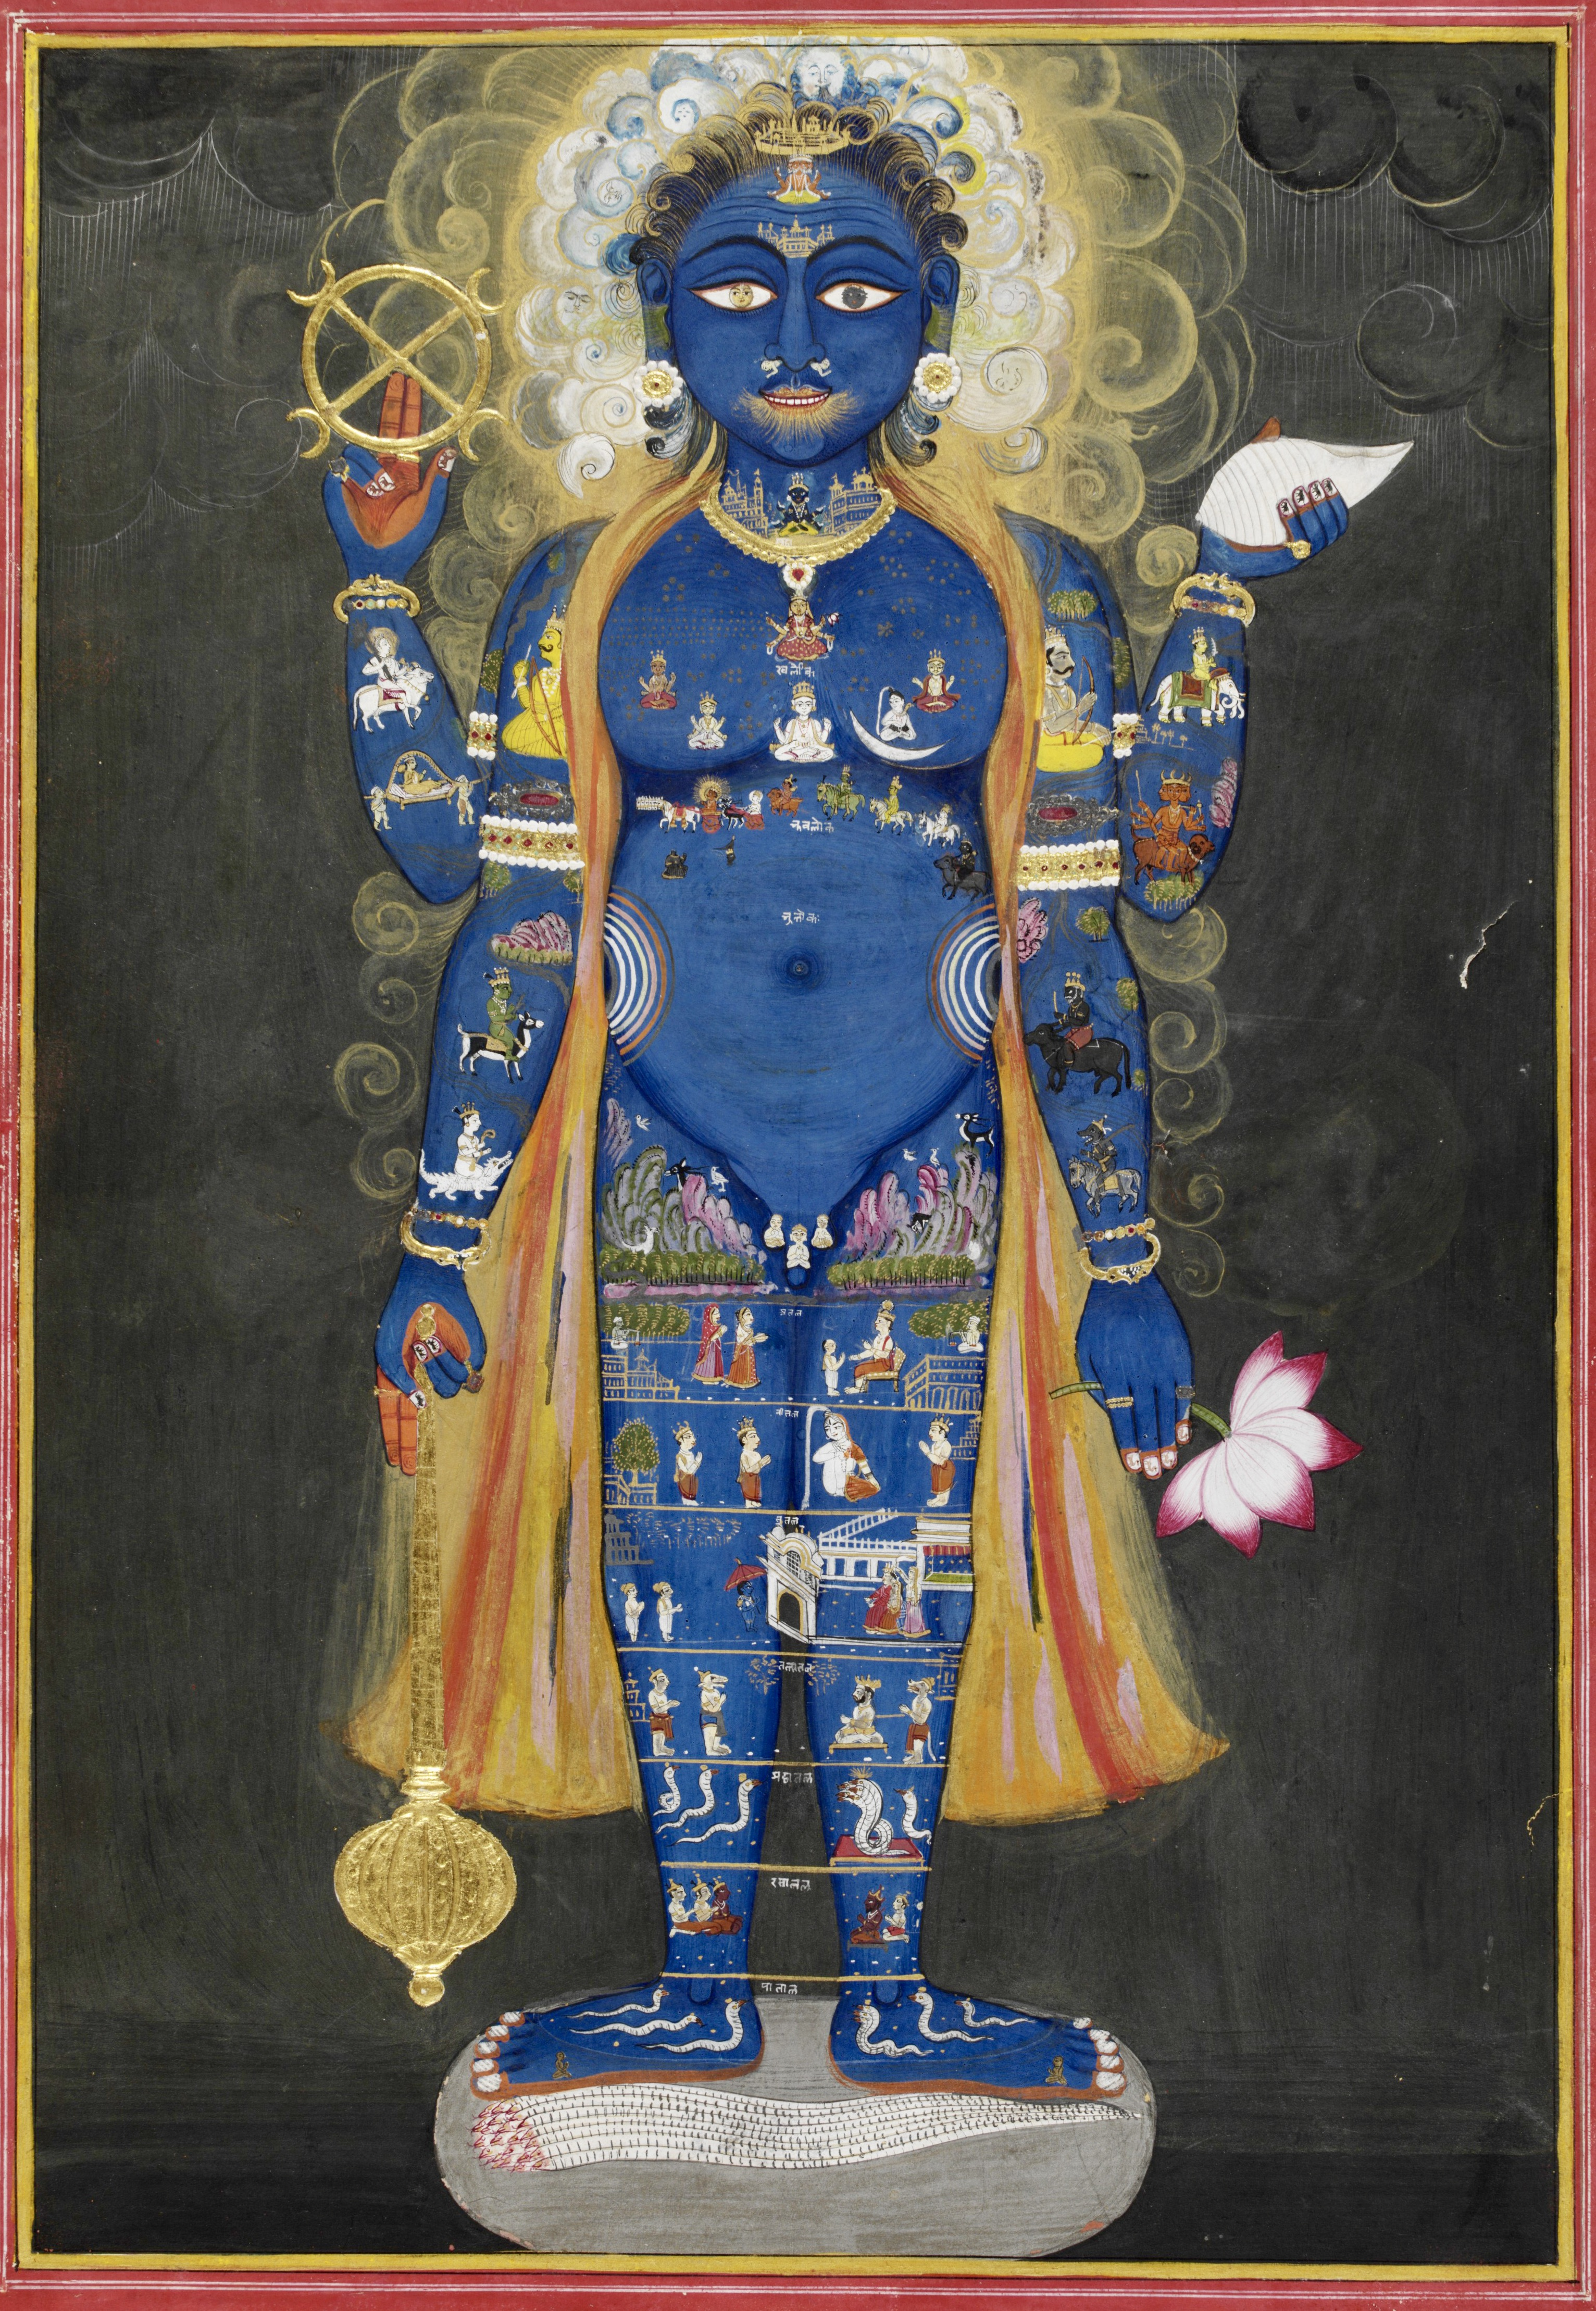
\includegraphics[width=1\textwidth]{pics/Vishnu_Vishvarupa_cropped.jpg}
	\caption{Viṣṇu Viśvarūpa, India, Rajasthan, Jaipur, ca. 1800–1820, Opaque watercolor and gold on paper, 38.5 × 28 cm, Victoria and Albert Museum, London, Given by Mrs. Gerald Clark.}
	\label{fig1}
      \end{figure}
\clearpage
  \begin{figure}[ht]
	\centering
  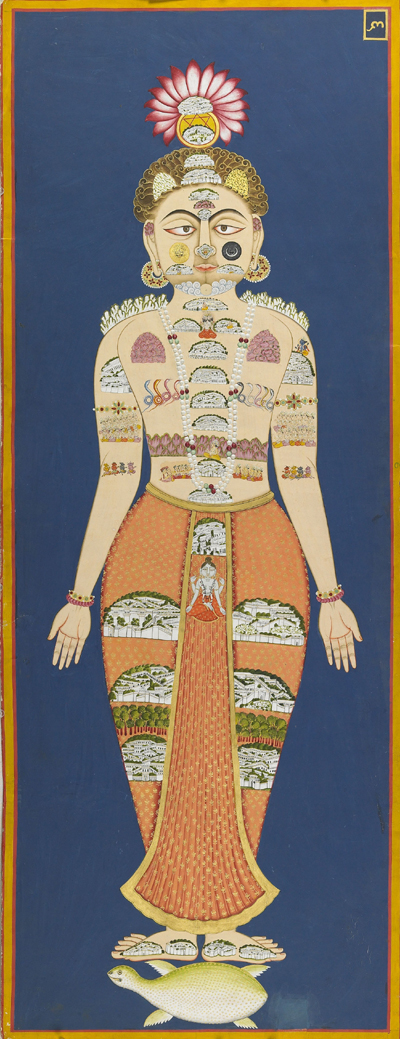
\includegraphics[width=0.5\textwidth]{pics/The_Equivalence_of_Self_and_Universe_(detail),_folio_6_from_the_Siddha_Siddhanta_Paddhati,_(Bulaki),_1824_(Samvat_1881);_122_x_46_cm._Mehrangarh_Museum_Trust..jpg}
	\caption{The Equivalence of Self and Universe (detail), folio 6 from the \textit{Siddhasiddhāntapaddhati} (Bulaki), India, Rajasthan, Jodhpur, 1824 (Samvat 1881), 122 x 46 cm, RJS 2378, Mehragarh Museum Trust.}
	\label{fig2}
      \end{figure}
      % \end{landscape}


\chapter{Bibliography}
 \label{sec:bibli}
   \clearpage
\newpage 
\thispagestyle{empty}
\quad  \addtocounter{page}{-1}

\printbibliography[heading=subbibintoc, title=Consulted Manuscripts, keyword=codex]

\printbibliography[heading=subbibintoc, title=Printed Editions, keyword=printsource]

\printbibliography[heading=subbibintoc, title=Secondary Literature, keyword=seclit]

\printbibliography[heading=subbibintoc, title=Online Sources, keyword=onlinesource]

\end{document}


